\chapter{Source detection as prior truncation} \label{cha:detection}

\todo{Rename as "Simulation-based inference for point sources"?}

Statistical inference of population parameters of astrophysical sources is challenging. It requires accounting for selection effects, which stem from the artificial separation between bright detected and dim undetected sources that is introduced by the analysis pipeline itself. In this chapter, we show that these effects can be modeled self-consistently in the context of sequential \gls*{sbi}. Our approach couples source detection and catalog-based inference in a principled framework that derives from the \gls*{tmnre} algorithm. It relies on the realization that detection can be interpreted as prior truncation. We outline the algorithm, and show first promising results.

\textit{This chapter is based on work from \cite{AnauMontel:2022ppb}.}


\section{Introduction}
\label{sec:ps-intro}

Point sources detection is crucial for astronomical surveys, and is the cornerstone for the compilation of source catalogues. Those source catalogues are then typically the basis for the inference of physical parameters that describe the sources at the population level. Upcoming astronomical facilities, such as the Square Kilometer Array (SKA)~\citep{Weltman:2018zrl} and the Cherenkov Telescope Array (CTA)~\citep{CTAConsortium:2017dvg} will deliver large and complex datasets.  In order to leverage their full potential, it is urgent to develop robust and automated source detection and source population parameters inference algorithms.

Machine learning is a particularly promising tool to address this big data challenge. Recent developments in deep learning and more generally automatic differentiation frameworks~\citep{baydin2018automatic} are increasingly used for tackling difficult astronomical data analysis with the goal to extricate more information from the available data. The capability of deep learning techniques of point sources detection and population characterization has been demonstrated across different wavelengths surveys, \eg~in $\gamma$-ray data~\citep{Panes:2021zig, Caron:2017udl, List:2021aer, Mishra-Sharma:2021oxe}, radio data~\citep{VafaeiSadr:2018tac, Rezaei:2021aa, Lukic:2019aa, Tilley:2020aa} and cosmic microwave background data~\citep{Bonavera:2021aa}.
In particular simulation-based machine learning approaches can be highly flexible, allowing to tailor developed pipelines to specific telescopes and science cases. 
A range of \gls*{sbi} algorithms have been proposed in the literature (see Ref.~\cite{Cranmer:2019eaq} for a review). An appealing feature is that they generally allow to directly estimate marginal posteriors for parameters of interest~\citep{Miller:2020hua}. Furthermore, \textit{sequential} \gls*{sbi} approaches~\citep{Durkan:2018aa, Papamakarios:2016ctj, Papamakarios:2018aa} have been shown to be particularly simulation efficient.  Among those, \gls*{tmnre} \citep{Miller:2020hua, Miller:2021aa} is a sequential \gls*{sbi} approach 
based on \gls*{nre}~\citep{Hermans:2019ioj},  which particularly well composes with marginalization.

\paragraph{Our contribution.}  Here, we present a strategy for how to use \gls*{tmnre} to simultaneously perform source detection and population-level parameters inference. This enables to self-consistently combine information from both detected and sub-threshold sources, without being affected by detection biases. The key idea is to recast the traditional concept of \emph{source detection} in terms of \emph{prior truncation}.  This will allow us to \textit{distill} information of bright sources directly into the simulation model. Our proposed method is highly interpretable since it resembles components of traditional survey analysis workflows. 


\section{Methodology}
\label{sec:ps-method}

We structure our methodology as follows. First, we introduce the problem setup, phrasing simulating point source maps in terms of a Bayesian hierarchical forward model in Section~\ref{subsec:ps-sim}. Secondly, in Section~\ref{subsec:ps-detection}, we perform point sources detection and estimate the point sources sensitivity function of our method. We then show how to include our catalogue of detected point sources in the forward model, recasting source detection as prior truncation, in Section~\ref{subsec:ps-truncation}. Lastly, we illustrate how to self-consistently perform point sources population parameters inference, by combining information from both detected and sub-threshold sources, in Section~\ref{subsec:ps-pop}. We show a schematic overview of the inference framework is shown in Figure~\ref{fig:ps-graphic}.

%  \subsection{Background}
%  
%\Gls*{tmnre} (and \gls*{nre} in general) performs posterior estimation by solving a binary classification problem. Given a model $p(x, z) = p(x\mid z) p(z)$, where $x$ is data, and $z$ a set of parameters of interest, one trains a network to distinguish joined samples $x, z \sim p(x, z)$ from marginal samples $x, z\sim p(x) p(z)$.  The networks learns to estimate the likelihood-to-evidence ratio $r(z; x)=p(x\mid z)/p(x)$
%  
%  which we can use to obtain weighted samples from the posterior $p(z \mid  x) = r(z; x) p(z)$.
%  %
%  %A key strength of \gls*{tmnre} is its scalability: the method targets only low-dimensional marginal posteriors, not joint, which are indispensable in likelihood-based inference (\eg~Markov chain Monte Carlo and variational simulation-based inference techniques).
%  %
%  In order to improve the network's learning and maximise the simulator efficiency, TMNRE concentrates in stages the regions in parameter space from which training examples are drawn based on a target observation. Hence, this truncation scheme restricts the prior distribution's support without modifying its shape, as opposed to other sequential methods that employ a posterior estimate as proposal distribution for generating simulations for the next round~\citep{Durkan:2018aa}.

\subsection{Problem setup} \label{subsec:ps-sim}

We consider here a simple Bayesian hierarchical source model,
  \begin{equation} \label{eq:ps-model}
    p(\data, \vec{\boldsymbol{s}}, \interest) = p(\data \mid  \vec{\boldsymbol{s}}) p(\interest) \prod_{i=1}^N p(\boldsymbol{s}_i\mid \interest)\;,
\end{equation}
where $\data$ is the observed sky map, $\boldsymbol{s}_i \equiv (F_i, \Omega_i)$ denotes the flux $F_i$ and position $\Omega_i$ of point source $i$, and $\interest \equiv \{N, \Sigma, h\}$ collects source population parameters, namely the number of sources $N$, and the parameters $\Sigma$ and $h$ that control the flux and spatial distributions respectively. To generate an observation, first, we sample point sources population parameters $\interest \equiv \{N, \Sigma, h\}$ from their priors, given in Table~\ref{tab:ps-model}. Then, for each point source, we draw its flux $F$ and position on the map $\Omega\equiv(l, b)$ from the priors given in Table~\ref{tab:ps-model}. We then generate a $128 \times 128$ pixels map. To model instrumental effects, we add a \gls*{psf} with Gaussian kernel standard deviation $\epsilon=1.5$ and Poisson noise, obtaining the final simulated map $\data$. We show examples of our simulated maps in the top row of the right panel of Figure~\ref{fig:ps-data}.
  
\begin{table}
  \centering
  \begin{tabular}{l l l }
    \toprule
        Parameter & & Prior \\
    \midrule
        Population parameters & & \\
            \quad number of point sources & $N$ & $\mathcal{U}(10, 500)$ \\
            \quad flux distribution parameter & $\Sigma$ & $\mathcal{U}(1, 3)$ \\
            \quad spatial distribution parameter & $h$ & $\mathcal{U}(1, 20)$ \\
    \midrule
        Point source parameters & & \\
            \quad flux & $F$ & $\mathcal{\log N}(1, \Sigma)$ \\
            \quad position & $\Omega\equiv(l, b)$ & ($\mathcal{N}(0, 20)$, $\mathcal{N}(0, h)$) \\
    \bottomrule
  \end{tabular}
  \caption{Point source simulation model parameters and priors.}
   \label{tab:ps-model}
\end{table}


\subsection{Source detection} \label{subsec:ps-detection}
For source detection we consider the following likelihood-to-evidence ratio,\footnote{
    \ In the following sections we will use the notation 
    $r(a; b\mid c) = \frac{p(a,b\mid c)}{p(a\mid c)p(b\mid c)}$, 
    where with `$\mid $' we refer to conditioning on specific variables for all factors in the ratio definition. If necessary, multiple variables are comma separated, for example $r(a, b; c\mid  d) = \frac{p(a, b, c\mid d)}{p(a, b\mid d)p(c\mid d)}$. Training conditional ratios is a straight-forward extension of \gls*{nre}, as seen in Section~\ref{subsec:anre-anre}.
}
\begin{equation}
    { r_1(\Omega, F_{th}; \data)} 
    \equiv \frac{
    p(\mathbb{I}_{\data}(F \geq F_{th})=1, \Omega\mid \data)
    }{
    p(\mathbb{I}_{\data}(F \geq F_{th})=1, \Omega)
    }\;.
    \label{eq:ps-rFth}
\end{equation}

Here, the denominator corresponds to the prior probability of having a source at position $\Omega$ with a flux $F\geq F_{th}$ that exceeds some threshold flux $F_{th}$.  The numerator is the corresponding posterior. We model the source detection ratio estimator in Equation~\eqref{eq:ps-rFth} as an image-to-image neural network that solves a binary classification problem in each image pixel. 
For simulated data, we call a simulated source $\boldsymbol{s}_i$ `detected' when there is a corresponding compact region as function of $\Omega$ where the detection significance is above threshold, ${ r_1(\Omega, F_{th}; \data)} > 5$. This effectively leads to a split between sources that are clearly identifiable and `sub-threshold' sources that are difficult to detect a individual instances.
Below, we assign the detection label $d_i = 1$ ($d_i = 0$) to detected (undetected) sources.

In order to characterize the split between detected and sub-threshold sources, we introduce a source-sensitivity function, $S(F, \Omega)$, which provides the probability that a source with flux $F$ and at position $\Omega$ would be detected by the ratio estimator in Equation~\eqref{eq:ps-rFth}.  This function can be estimated by training the ratio estimator
\begin{equation}
    { r_2(d;F, \Omega, \data)}
    \equiv \frac{p(d\mid  F, \Omega, \data)}
    {p(d)}
    \label{eq:ps-rd}
\end{equation}
which is marginalised over all other sources and source parameters. By omitting the dependence on the map, $\data$, which is then effectively marginalized, the ratio estimator can then simply be modeled as a $\mathbb{R}^3 \to \mathbb{R}$ \gls*{mlp}. The source-sensitivity function can then be estimated as 
\begin{equation}
S(F, \Omega) = \sigma\left(\log \left(\frac{p(d=1\mid F, \Omega)}{p(d=0\mid F, \Omega)}\right)\right),
\end{equation}
where we have introduced the sigmoid function $\sigma(y) \equiv 1 / (1 + e^{-y})$. 

Once we know the sensitivity function $S(F, \Omega)$, we can make the concept of source detection part of our model as follows.  In a random realization, each source $i$ will be either detected, $d_i= 1$ (with probability $S(F_i, \Omega_i)$), or not detected, $d_i=0$ (with probability $1-S(F_i, \Omega_i)$).  To keep notation simple, we omit $d_i$ and instead group detected and non-detected (sub-treshold) sources together in vectors with corresponding subscripts, and write $\vec{\boldsymbol{s}} \equiv (\vec{\boldsymbol{s}}_{det}, \vec{\boldsymbol{s}}_{sub})$.
Taking into consideration this split, our model becomes
\begin{equation}
    p(\data, \vec{\boldsymbol{s}}_{det}, \vec{\boldsymbol{s}}_{sub}, \interest) = p(\data\mid  \vec{\boldsymbol{s}}_{det}, \vec{\boldsymbol{s}}_{sub})
    p(\vec{\boldsymbol{s}}_{det}\mid \interest) 
    p(\vec{\boldsymbol{s}}_{sub}\mid \interest) 
    p(\interest)\;.
    \label{eq:ps-splitmodel}
\end{equation}

Importantly, although $p(\vec{\boldsymbol{s}}_{det/sub}\mid \interest)$ depends on the sensitivity function $S(F_i, \Omega_i)$, the distribution of all sources $p(\vec{\boldsymbol{s}}\mid \interest)$ is the same as in Equation~\eqref{eq:ps-model}.


\subsection{Detection as truncation} \label{subsec:ps-truncation}

Finally, we introduce our truncation scheme. 
Truncating source priors in Equation~\eqref{eq:ps-model} is difficult due to the the label switching problem ($\data$ is invariant under relabeling sources). However, once specific sources are detected, they can be labeled and ordered arbitrarily. Let us assume that $N_{det}$ sources were detected by the ratio estimator in Equation~\eqref{eq:ps-rFth} in the regions $\mathcal{R}_i$ with $i = 1, \dots, N_{det}$ for a given observation of reference $\data_o$.  Our ansatz for the indicator function, which selects a specific prior region, is
\begin{equation}
    \mathbb{I}_{\data_o}(\vec{\boldsymbol{s}}_{det}) = \prod_{i=1}^{N_{det}}
    \mathbb{I}_{\data_o}(\Omega_i \in \mathcal{R}_i)
    \mathbb{I}_{\data_o}(F_i \geq F_{th})\;.
    \label{eq:ps-I}
\end{equation}

Our truncation strategy is now to focus on the parameter space where $\mathbb{I}_{\data_o}(\vec{\boldsymbol{s}}_{det})=1$ for our data of interest $\data_o$, in order to reduce training data variance. 
We can then write our truncated model as 
\begin{equation}\label{eq:ps-truncatedmodel}
  \centering
\begin{split}
    p(\data, &\vec{\boldsymbol{s}}_{det}, \vec{\boldsymbol{s}}_{sub}, \interest,
    \mathbb{I}_{\data_o}(\vec{\boldsymbol{s}}_{det}))  \\ 
    &= p(\data\mid  \vec{\boldsymbol{s}}_{det}, \vec{\boldsymbol{s}}_{sub})
    p(\vec{\boldsymbol{s}}_{det}\mid \interest,\mathbb{I}_{\data_o}(\vec{\boldsymbol{s}}_{det}))
    p(\vec{\boldsymbol{s}}_{sub}\mid \interest) 
    p(\interest)
    p(\mathbb{I}_{\data_o}(\vec{\boldsymbol{s}}_{det})\mid \interest) \; ,
\end{split}
\end{equation}
where detected sources $p(\vec{\boldsymbol{s}}_{det})$ can be sampled only in the relevant parameter space  $\mathbb{I}_{\data_o}(\vec{\boldsymbol{s}}_{det})=1$ .

\subsection{Population parameters inference with truncation}  \label{subsec:ps-pop}
Given some observation $\data_o$, we want to estimate the posterior $p(\interest\mid \data_o)$. Since the truncation affects parameters $\vec{\boldsymbol{s}}_{det}$ whose prior depends on population parameters $\interest$, the truncation volume is not a constant factor, and the procedure requires extra care. We can estimate the posterior $p(\interest\mid \data)$ by considering the ratio
\begin{equation}\label{eq:ps-posterior}
\centering
\begin{split}
    r(\interest; \data) &= \cfrac{p(\interest\mid \data)}{p(\interest)} \simeq \cfrac{p(\interest\mid \data, \mathbb{I}_{\data_o}(\vec{\boldsymbol{s}}_{det})=1)}{p(\interest)} \\
    &= 
    \underbrace{\frac{p(\interest\mid \data, \mathbb{I}_{\data_o}(\vec{\boldsymbol{s}}_{det})=1)}{p(\interest\mid \mathbb{I}_{\data_o}(\vec{\boldsymbol{s}}_{det})=1)}}_{\equiv { r_3(\interest; \data\mid \mathbb{I}_{\data_o}(\vec{\boldsymbol{s}}_{det})=1)}}
    \underbrace{\frac{p(\interest\mid \mathbb{I}_{\data_o}(\vec{\boldsymbol{s}}_{det})=1)}{p(\interest)}}_{\equiv
    r(\interest; \mathbb{I}_{\data_o}(\vec{\boldsymbol{s}}_{det})=1)}\;.
\end{split}
\end{equation}

The second step in Equation~\eqref{eq:ps-posterior} corresponds to the truncation approximation. It is exact (in the sense of leaving $p(\interest\mid \data_o)$ unaffected) in the limit where $p(\data_o\mid \mathbb{I}_{\data_o}(\vec{\boldsymbol{s}}_{det})=0) \to 0$. It exploits the fact that $\mathbb{I}_{\data_o}(\vec{\boldsymbol{s}}_{det}) = 1$ does not add information beyond what is already known from $\data_o$.  
Training that ratio estimator directly with \gls*{tmnre} would be challenging since $\mathbb{I}_{\data_o}(\vec{\boldsymbol{s}}_{det})=1$ has very small support in the training data.  Instead, we split the ratio into two computationally feasible ratios (this is in spirit similar to the telescoping ratio estimation approach presented in Ref.~\cite{Rhodes:2020aa}).

The first ratio, $ r_3(\interest; \data\mid \mathbb{I}_{\data_o}(\vec{\boldsymbol{s}}_{det})=1)$, can be estimated by training a peak-count network~\citep{Cholakkal:2019aa, Ranjan:2021aa, Kilic:2021aa} on targeted data, that is truncated to $\mathbb{I}_{\data_o}(\vec{\boldsymbol{s}}_{det})=1$. The second ratio can be estimated as
\begin{equation}\label{eq:ps-average}
\begin{split}
    r(\interest; \mathbb{I}_{\data_o}(\vec{\boldsymbol{s}}_{det})=1)
    &= \frac{p(\interest\mid \mathbb{I}_{\data_o}(\vec{\boldsymbol{s}}_{det})=1)}{p(\interest)}
    = \frac{p(\mathbb{I}_{\data_o}(\vec{\boldsymbol{s}}_{det})=1\mid \interest)}{p(\mathbb{I}_{\data_o}(\vec{\boldsymbol{s}}_{det})=1)}\\
    &= \int d\vec{\boldsymbol{s}}_{det} \frac{p(\vec{\boldsymbol{s}}_{det}\mid \interest)} {p(\vec{\boldsymbol{s}}_{det})}
    \frac{p(\vec{\boldsymbol{s}}_{det})\mathbb{I}_{\data_o}(\vec{\boldsymbol{s}}_{det})}{p(\mathbb{I}_{\data_o}(\vec{\boldsymbol{s}}_{det})=1)} \\
    &= \int d\vec{\boldsymbol{s}}_{det} 
    \underbrace{\frac{p(\vec{\boldsymbol{s}}_{det}\mid \interest)} {p(\vec{\boldsymbol{s}}_{det})}}_{
    \equiv {r_4(\vec{\boldsymbol{s}}_{det};\interest)}}
    p(\vec{\boldsymbol{s}}_{det}\mid \mathbb{I}_{\data_o}(\vec{\boldsymbol{s}}_{det})= 1) \; ,
\end{split}
\end{equation}
so it can be estimated by training a network on detected sources lists on un-truncated training data.
In practice, we generate weighted samples from the full posterior $p(\interest\mid \data)$ by sampling $\interest, \vec{\boldsymbol{s}}_{det} \sim p(\interest)p(\vec{\boldsymbol{s}}_{det}\mid \mathbb{I}_{\data_o}(\vec{\boldsymbol{s}}_{det})=1)$
with weights
$w = { r_3(\interest; \data\mid \mathbb{I}_{\data_o}(\vec{\boldsymbol{s}}_{det})=1)}\cdot
r(\interest; \mathbb{I}_{\data_o}(\vec{\boldsymbol{s}}_{det})=1)
%{ r_4(\vec{\boldsymbol{s}}_{det}; \interest)}
$.  

In the process, we trained four ratio estimation networks that are directly connected with traditional source analysis pipeline components: $ r_1(\Omega, F_{th}; \data)$ performs source detection; $r_2(d; F, \Omega, \data)$ is the source sensitivity function; $ r_3(\interest; \data\mid \mathbb{I}_{\data_o}(\vec{\boldsymbol{s}}_{det})=1)$ constraints $\interest$ based on sub-threshold sources (because detected sources are assumed to be fixed in the parameter space where $\mathbb{I}_{\data_o}(\vec{\boldsymbol{s}}_{det})=1$); and $r_4(\vec{\boldsymbol{s}}_{det}; \interest)$ constraints $\interest$ using the detected sources catalog.
We show a schematic overview of the inference framework used in this work in Figure~\ref{fig:ps-graphic}.

\begin{figure}
    \centering
    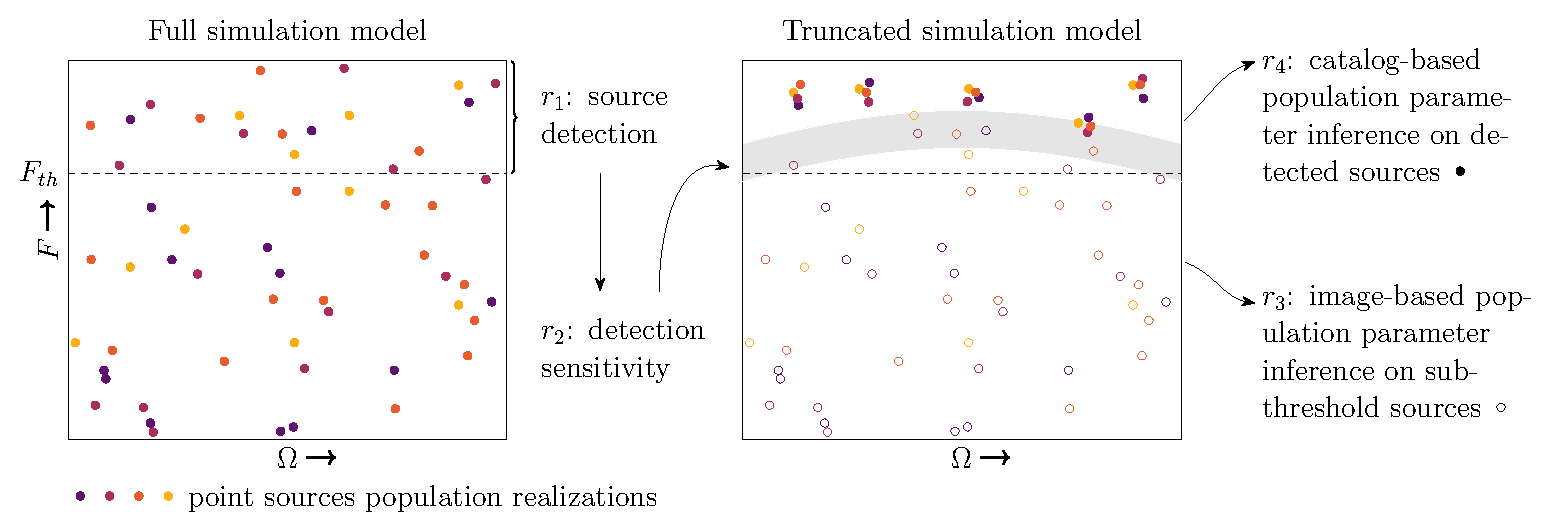
\includegraphics[width=\linewidth]{PS-graphic.pdf}
    \caption{Illustration of our inference framework (see Section~\ref{sec:ps-method} for details). \textit{Left panel}: A source detection network $r_1$ and the corresponding sensitivity network $r_2$ are trained based on the full simulation model. \textit{Right panel}: Bright sources are constrained in the truncated simulation model, while sub-threshold sources vary freely.  Two inference networks are trained to capture information from sub-threshold sources ($r_3$) and detected sources ($r_4$).
    }
    \label{fig:ps-graphic}
\end{figure}


\section{Experiment}
\label{sec:ps-results}

\begin{figure}
    \centering
    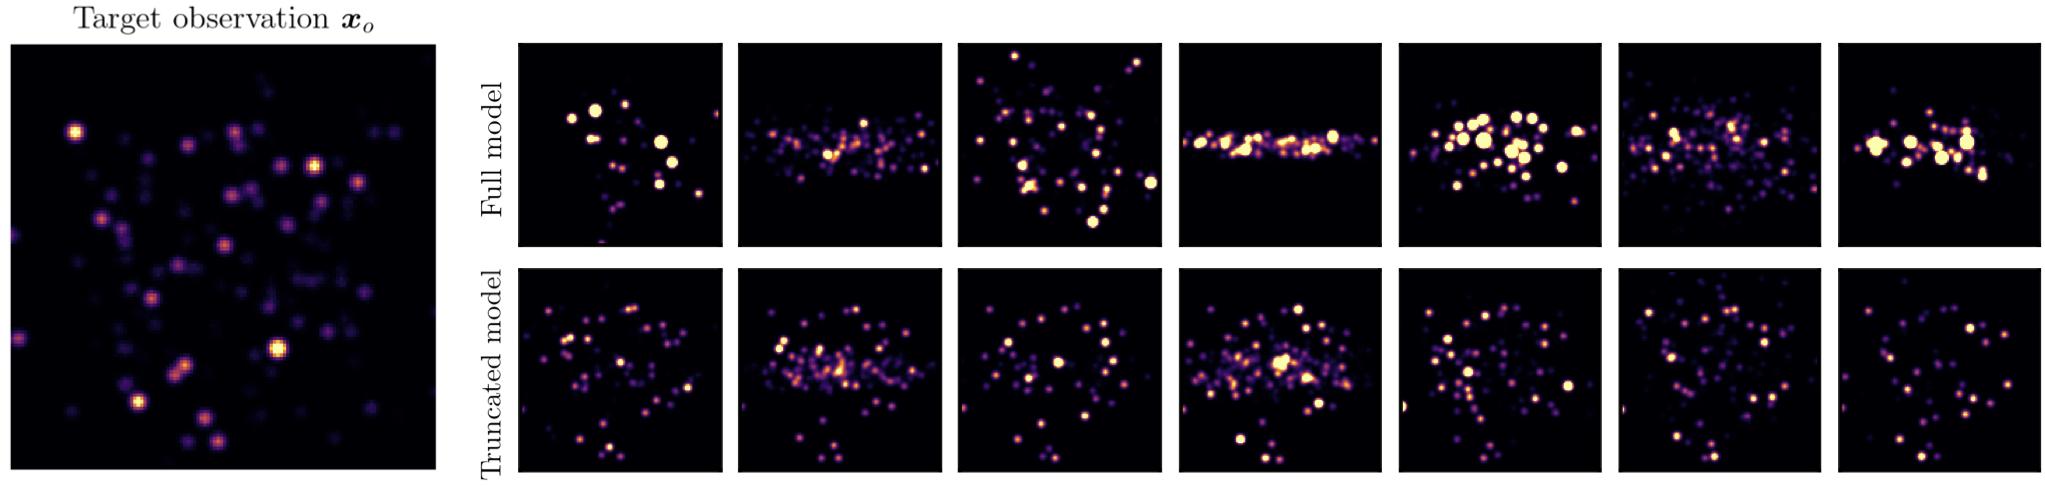
\includegraphics[width=\linewidth, clip=true, trim = 0mm 0mm 16cm 0mm]{PS-data.jpg}
    \caption{
      \textit{Left:} Observation of reference $\data_o$. 
      \textit{Right:} In the first row we show samples from our full simulation model. In the second row we show targeted samples from the truncated model. Targeted data are visually more close to $\data_o$, the main dissimilarities are due to different sub-threshold sources and instrumental effects realizations.
    }
    \label{fig:ps-data}
\end{figure}

\begin{figure}
    \centering
    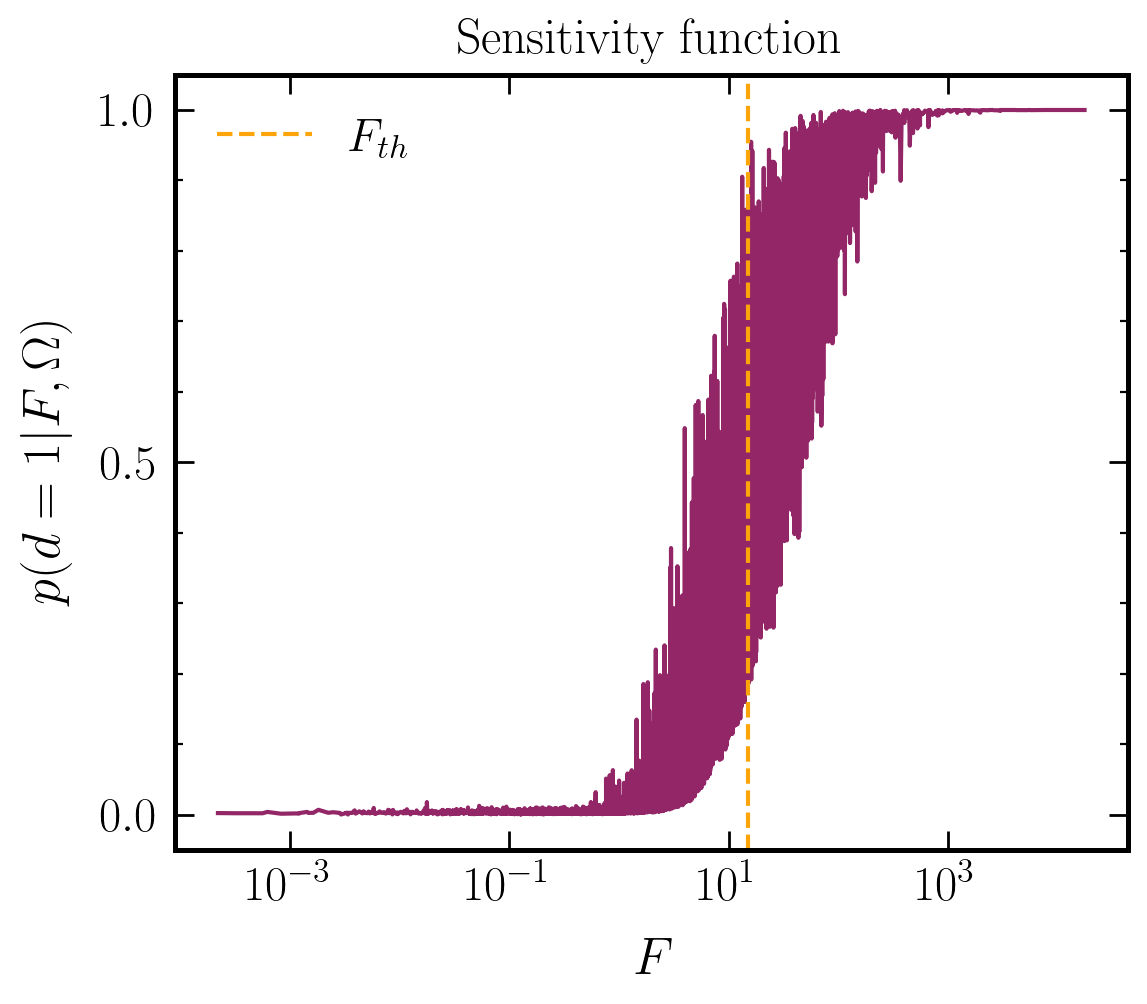
\includegraphics[width=0.6\linewidth]{PS-sensitivity.png}
    \caption{Point source sensitivity function $S(F, \Omega)$ as a function of flux $F$. The function characterizes the split between detected and sub-threshold sources by the source detection network $r_1$, providing the probability that a source with flux $F$ and at position $\Omega$ would be detected by the ratio estimator in Equation~\eqref{eq:ps-rFth}.  
    }
    \label{fig:ps-sensitivity}
\end{figure}

\begin{figure}
\centering
      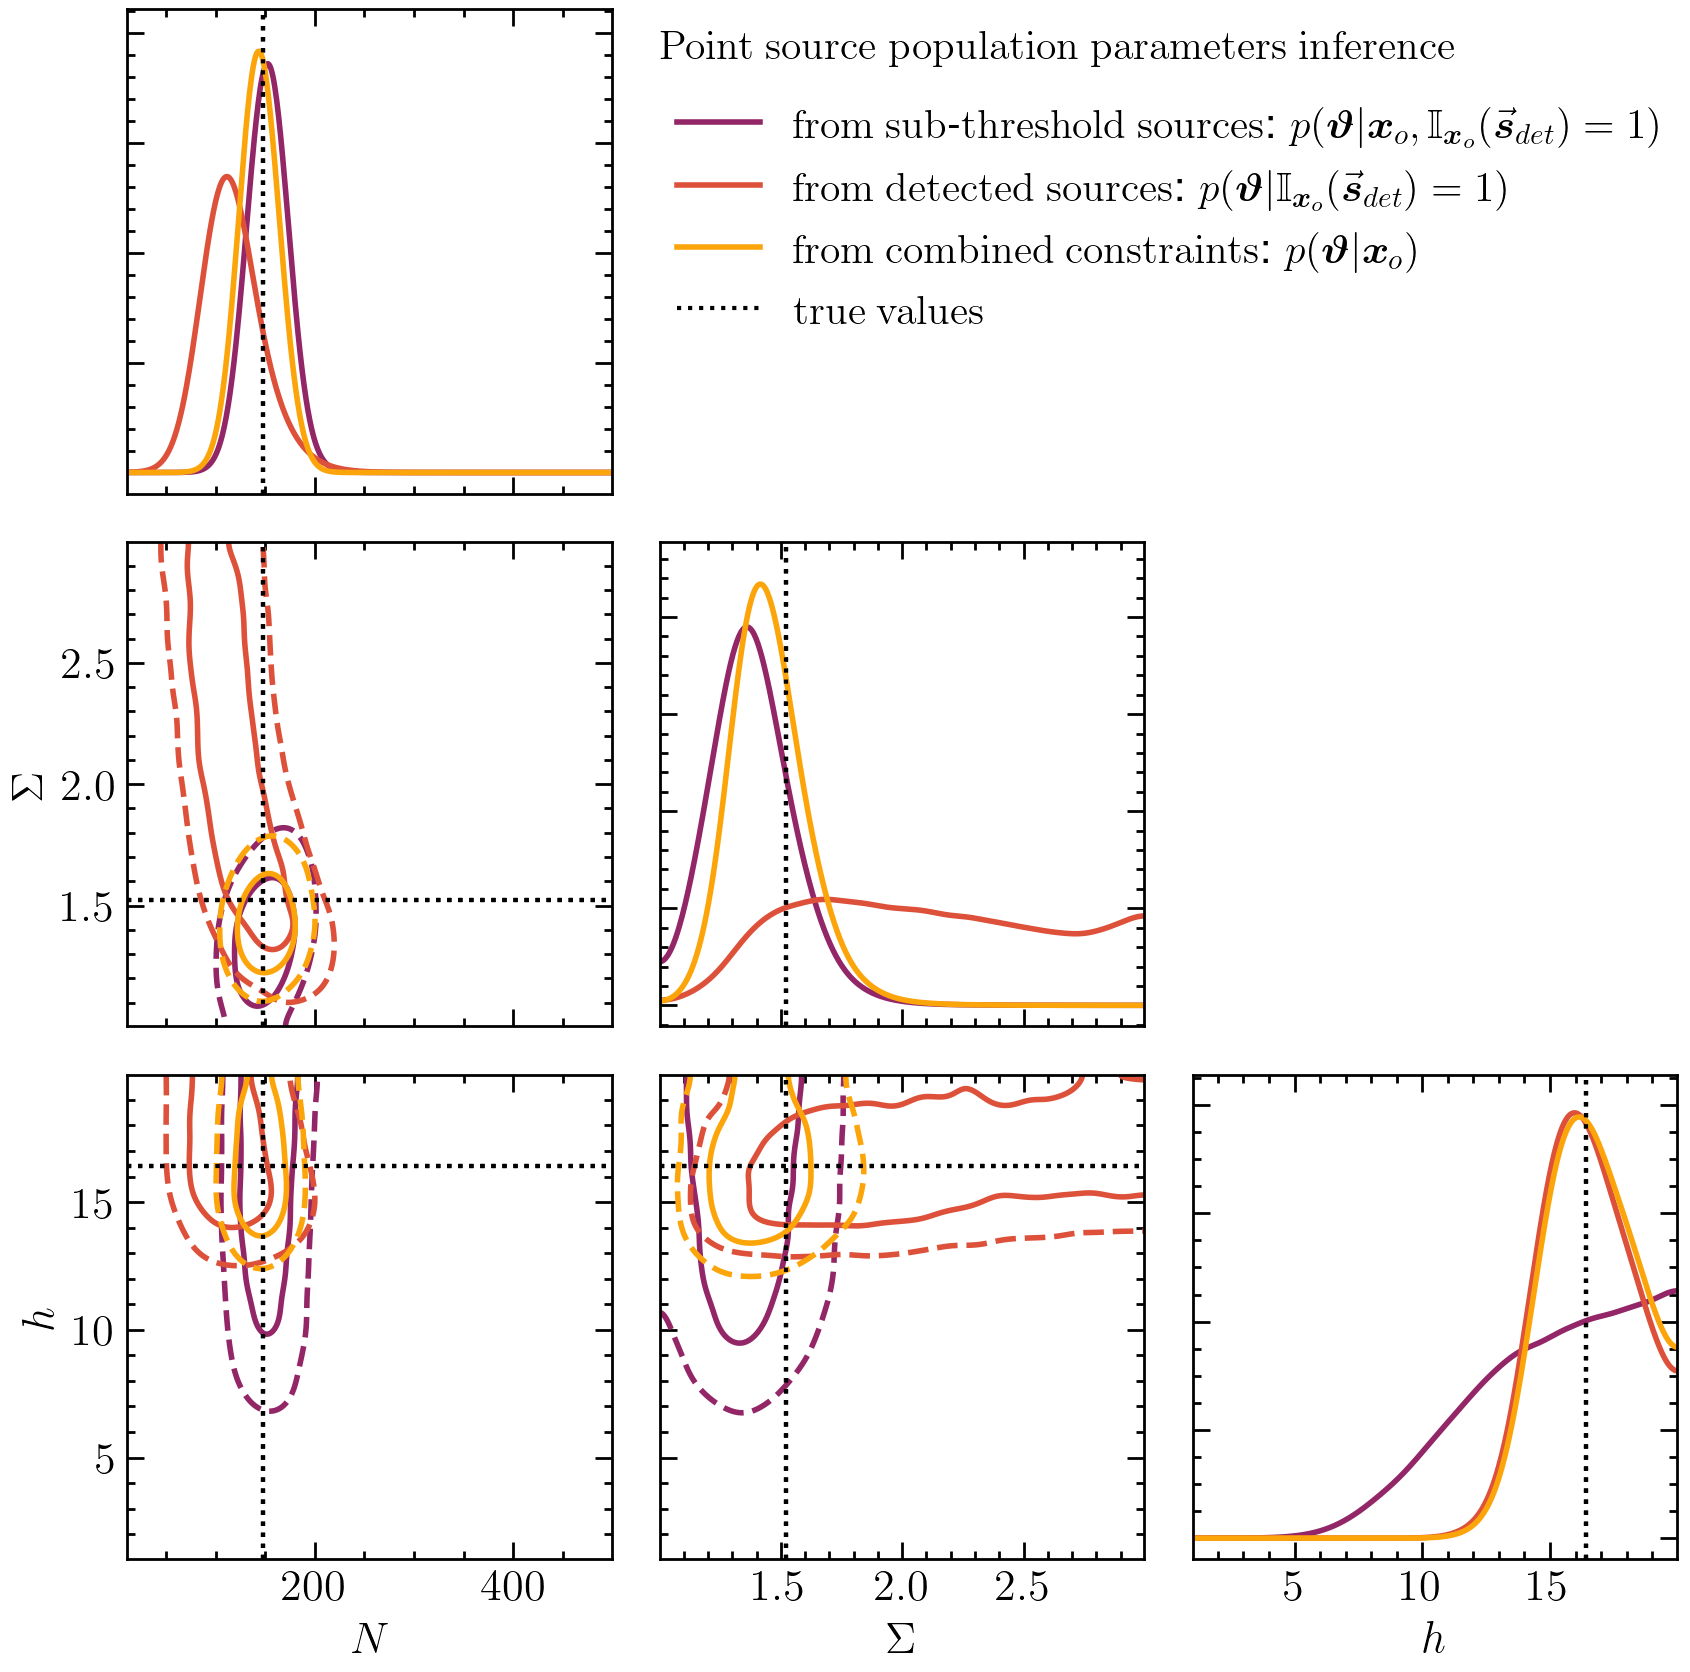
\includegraphics[width=0.75\linewidth]{PS-results.jpg}
    \caption{Marginal posteriors inferred by \gls*{tmnre} on target observation $\data_o$ for population parameters $\interest$. We show constraints from sub-threshold sources (violet), detected sources (orange), and combined results (yellow). In the 2D marginal posterior we indicate the $68\%$ and $95\%$ credible regions with solid and dashed lines respectively. For more details see Section~\ref{sec:ps-results}.
}
\label{fig:ps-results}
\end{figure}

We apply the proposed methodology to the simulated target observation $\data_o$ shown in Figure~\ref{fig:ps-data}. 

\paragraph{Training strategy.} We first train the source detection ratio estimator in Equation~\eqref{eq:ps-rFth} on data simulated from the full model shown in Equation~\eqref{eq:ps-model}, and then apply it to $\data_o$ to obtain a detection map. From the detection map we derive a catalog of detected sources $\vec{\boldsymbol{s}}_{det}$, and define a truncated parameter space of interest, where $\mathbb{I}_{\data_o}(\vec{\boldsymbol{s}}_{det})=1$. In order to make source detection part of our model, we train the sensitivity ratio estimator in Equation~\eqref{eq:ps-rd} to estimate the sensitivity function $S(F, \Omega)$, illustrated in Figure~\ref{fig:ps-sensitivity}. We then generate targeted training data from our truncated simulation model in Equation~\eqref{eq:ps-truncatedmodel}. We show samples from the full model and the truncated one in Figure~\ref{fig:ps-data}. Finally, we train two inference networks to capture information regarding population parameters from sub-threshold and detected sources, as explained in Section~\ref{sec:ps-method}. 
The four neural networks were trained on a NVIDIA GeForce RTX 3080 Ti GPU, the total computational time cost to obtain the results shown in Figure~\ref{fig:ps-results} is $\sim 2$ hours. 

\paragraph{Results.} We show the constraints on population parameters $\interest$  from sub-threshold sources, detected ones, and their combination in Figure~\ref{fig:ps-results}. The different posteriors are consistent with each other, indicating that the proposed inference framework automatically accounts for detection biases. We see that different constraints are dominated by different neural networks, \eg~the number $N$ of point source is better constrained by sub-threshold ones, whereas the spatial distribution parameter $h$ by detected ones. The weaker constraint on the flux parameter $\Sigma$ inferred from detected sources is due to the fact that in Equation~\eqref{eq:ps-average} we average over different detected sources realisations, always re-sampling the parameter $\Sigma$ (see Section~\ref{subsec:ps-sim} for the hierarchical model details).


\section{Discussion and conclusions}
\label{sec:ps-conclusions}

We have introduced a novel method to self-consistently perform point sources detection and source population parameters inference using \gls*{tmnre}. The key realization underlying this methodology is that point source detection is equivalent to prior truncation and essential to reduce training data variance. With this approach, we can exploit information of detected as well as sub-threshold sources for population-level parameter inference. Detection biases are automatically accounted for in our approach. Exemplary results of our approach are presented in Figure~\ref{fig:ps-results}, where we show inference results on source population parameters from both detected point sources and sub-threshold sources separately, as well as their combination. 

Since the proposed method is essentially a specific implementation of  \gls*{tmnre}, we expect that it inherits its positive properties in terms of simulation-efficiency and scalability \cite{Miller:2021aa}. A possible shortcoming of this approach is that multiple neural networks need to be trained self-consistently, which on the other hand have a clear interpretation in terms of traditional analysis pipeline components. A potential application beyond those directly intended is to detectable and sub-threshold substructures in strong gravitational lenses.


%  \paragraph{Broader Impact}
%  \label{par:impact}
%  This work is focusing on the analysis of astronomical surveys that contain point sources population via TMNRE. Variants of the presented approach could find application in other areas of the physical sciences. We do not expect any negative societal impact of the presented methods. However, we recommend the usual caution in inferring scientific conclusions based on a complex methodology.

  
%  \section*{Acknowledgments and Disclosure of Funding}
%  
%  This work is part of a project that has received funding from the European Research Council (ERC) under the European Union’s Horizon 2020 research and innovation program (Grant agreement No. 864035 -- Undark).
%  
%  We acknowledge the use of the \texttt{python} \citep{python} modules, \texttt{matplotlib} \citep{Hunter:2007ouj}, \texttt{numpy} \citep{Harris:2020xlr},  \texttt{scipy} \citep{Virtanen:2019joe}, \texttt{PyTorch} \citep{pytorch}, \texttt{tqdm} \citep{tqdm}, and \texttt{jupyter} \citep{jupyter}.

  
